\documentclass[11pt,a4paper]{article}

% -------------------------------
% Packages
% -------------------------------
\usepackage[utf8]{inputenc}
\usepackage[T1]{fontenc}
\usepackage{lmodern}
\usepackage{geometry}
\geometry{margin=1in}

\usepackage{amsmath,amssymb}
\usepackage{tikz}
\usetikzlibrary{shapes.geometric, arrows.meta, positioning, calc}
\usepackage{graphicx}
\usepackage{float}
\usepackage{adjustbox}

% -------------------------------
% Colours (matching your SVG/TikZ theme)
% -------------------------------
\definecolor{boxFill}{HTML}{F2F7FF}
\definecolor{boxStroke}{HTML}{3366CC}
\definecolor{procFill}{HTML}{E8FFF2}
\definecolor{procStroke}{HTML}{33AA55}
\definecolor{lossFill}{HTML}{FFF2E6}
\definecolor{lossStroke}{HTML}{FF9933}

\title{PROJECT ROADMAP\\Hybrid Selective Kernel Self-Supervised Acoustic Representation Learning System}
\author{}
\date{}

\begin{document}
\maketitle

% =================================================
\section*{1. Initial Sample Creation (Stage -1)}

Objective: Provide raw waveform inputs for the system before Stage 0 begins.
This stage is external to the main ML pipeline and is part of the Dataset Plan (non-pipeline).

Tasks: Generate synthetic vessel-noise waveforms using a Python-based generator.
\begin{itemize}
\item Produce physics-inspired acoustic signatures including blade-rate tonals, multi-harmonics, broadband propulsion noise, cavitation bursts, and Doppler-induced warping.
\item Save the generated signals as \texttt{.wav} files at the standard sampling rate of 16 kHz.
\item Organise the synthetic dataset into labeled vessel-type folders.
\end{itemize}

Output: A set of initial waveform files (e.g., \texttt{.wav}) ready for ingestion by Stage 0 (Preprocessing).

Note: This stage does not replace real-world datasets. It exists to support early debugging, model bring-up, augmentation testing, and baseline evaluation before integrating NOAA, MBARI, JAMSTEC, or DCLDE datasets.

% =================================================
\section*{2. Stage 0 — Preprocessing \& Data Standardisation}

Objective: Ensure all raw signals are consistent, normalised, and ready for model ingestion.

Tasks:
\begin{itemize}
\item Resample audio to a fixed sampling rate.
\item Remove DC offset.
\item Apply amplitude normalisation.
\item Optional high-pass filter.
\item Silence trimming / energy-gated cropping.
\item Segment into fixed-length clips.
\end{itemize}

Output: Tensor \texttt{[Batch, 1, T]}

% =================================================
\section*{3. Stage 1 — Learned Filterbank (Raw Waveform Front-End)}

Objective: Replace STFT/mel spectrogram preprocessing with a learned multi-scale time-domain filterbank.

Design:
\begin{itemize}
\item Multi-branch SKConv1D with kernels (3,5,7,11,15).
\item Optional dilated kernels.
\item Optional initial Conv1D (kernel 512, stride 256).
\end{itemize}

Output: \texttt{[B, F, T1]} Learned time--feature map.

Phenomena Captured: Transients, tonals, modulation, broadband noise.

% =================================================
\section*{4. Stage 2 — Hierarchical 2D Acoustic Encoder}

Objective: Convert learned time--feature map into high-level 2D embeddings.

Workflow:
\begin{itemize}
\item Reshape \texttt{[B, F, T1]} $\rightarrow$ \texttt{[B,1,F,T1]}
\item Apply SKConv2D blocks
\item Global pooling
\item Linear projection to $h \in \mathbb{R}^{D}$
\end{itemize}

% =================================================
\section*{5. Stage 3 — Self-Supervised Representation Learning (SSL)}

Objective: Train encoder without labels using Barlow Twins.

Components:
\begin{itemize}
\item Siamese encoder with shared weights.
\item Projector head $g(h)$.
\item Barlow Twins loss: invariance + decorrelation.
\item Optional: SimCLR, VICReg.
\end{itemize}

% =================================================
\section*{6. Stage 4 — Data Pipeline \& Augmentation Engine}

Objective: Generate physics-consistent positive pairs.

Augmentations:
\begin{itemize}
\item Random crop
\item Time shift
\item Gain jitter
\item Gaussian noise
\item Band-pass / low-pass filters
\item Time masking
\item Optional: Frequency masking
\end{itemize}

% =================================================
\section*{7. Stage 5 — Training, Embedding Extraction \& Clustering}

Training Loop: Augment $\rightarrow$ Encode $\rightarrow$ Project $\rightarrow$ Loss $\rightarrow$ Update.

Embedding Extraction: Discard projector, optional PCA/whitening.

Clustering: HDBSCAN (preferred), DBSCAN (alternative).

Visualisation: UMAP, t-SNE, cluster averages.

% =================================================
\section*{8. Stage 6 — Optional / Recommended Extensions}

\begin{itemize}
\item Evaluation \& analytics
\item Embedding variance diagnostics
\item Invariance robustness tests
\item Correlation heatmaps
\end{itemize}

% =================================================
\section*{9. Stage 7 — Deployment \& Export}

\begin{itemize}
\item ONNX export for embedded inference
\item Optional quantisation
\item Deploy to ARM/DSP hardware
\end{itemize}

% =================================================
\section*{10. Deliverables (Non-Pipeline)}

\begin{itemize}
\item SKConv1D implementation
\item SKConv2D implementation
\item HybridSKEncoder
\item SSL wrapper
\item Augmentation engine
\item Training pipeline
\item Clustering utilities
\item ONNX export
\item Full TDD
\end{itemize}

% =================================================
\section*{11. Dataset Plan (Non-Pipeline)}

For initial testing, the system will use a Synthetic Vessel Noise Generator implemented in Python.
This generator produces physics-inspired vessel acoustic signatures (blade-rate tonals, broadband noise,
cavitation bursts, Doppler-shifted modulations), enabling controlled validation of the SKConv1D and
SKConv2D architecture.

For subsequent evaluation using real-world underwater acoustic signals, the following publicly accessible datasets will be used:
\begin{itemize}
\item NOAA NCEI Passive Acoustic Archives -- Real hydrophone recordings containing vessel noise.
\item MBARI Hydrophone Dataset -- Includes vessel pass-bys, maritime traffic, and ambient underwater noise.
\item JAMSTEC Underwater Observatory Recordings -- Long-term hydrophone deployments with merchant ship noise.
\item DCLDE Workshop Datasets -- Include mixed marine mammal and vessel acoustic events suitable for SSL validation.
\end{itemize}

These datasets provide diverse underwater vessel noise signatures required for unsupervised clustering,
embedding evaluation, and robustness benchmarking.

% =================================================
\section*{12. Flowchart Diagram}

(See System Flowchart (Authoritative).)

\clearpage
\section*{System Flowchart (Authoritative)}

\begin{figure}[H]
\centering
\begin{adjustbox}{max totalsize={\textwidth}{0.90\textheight},center}
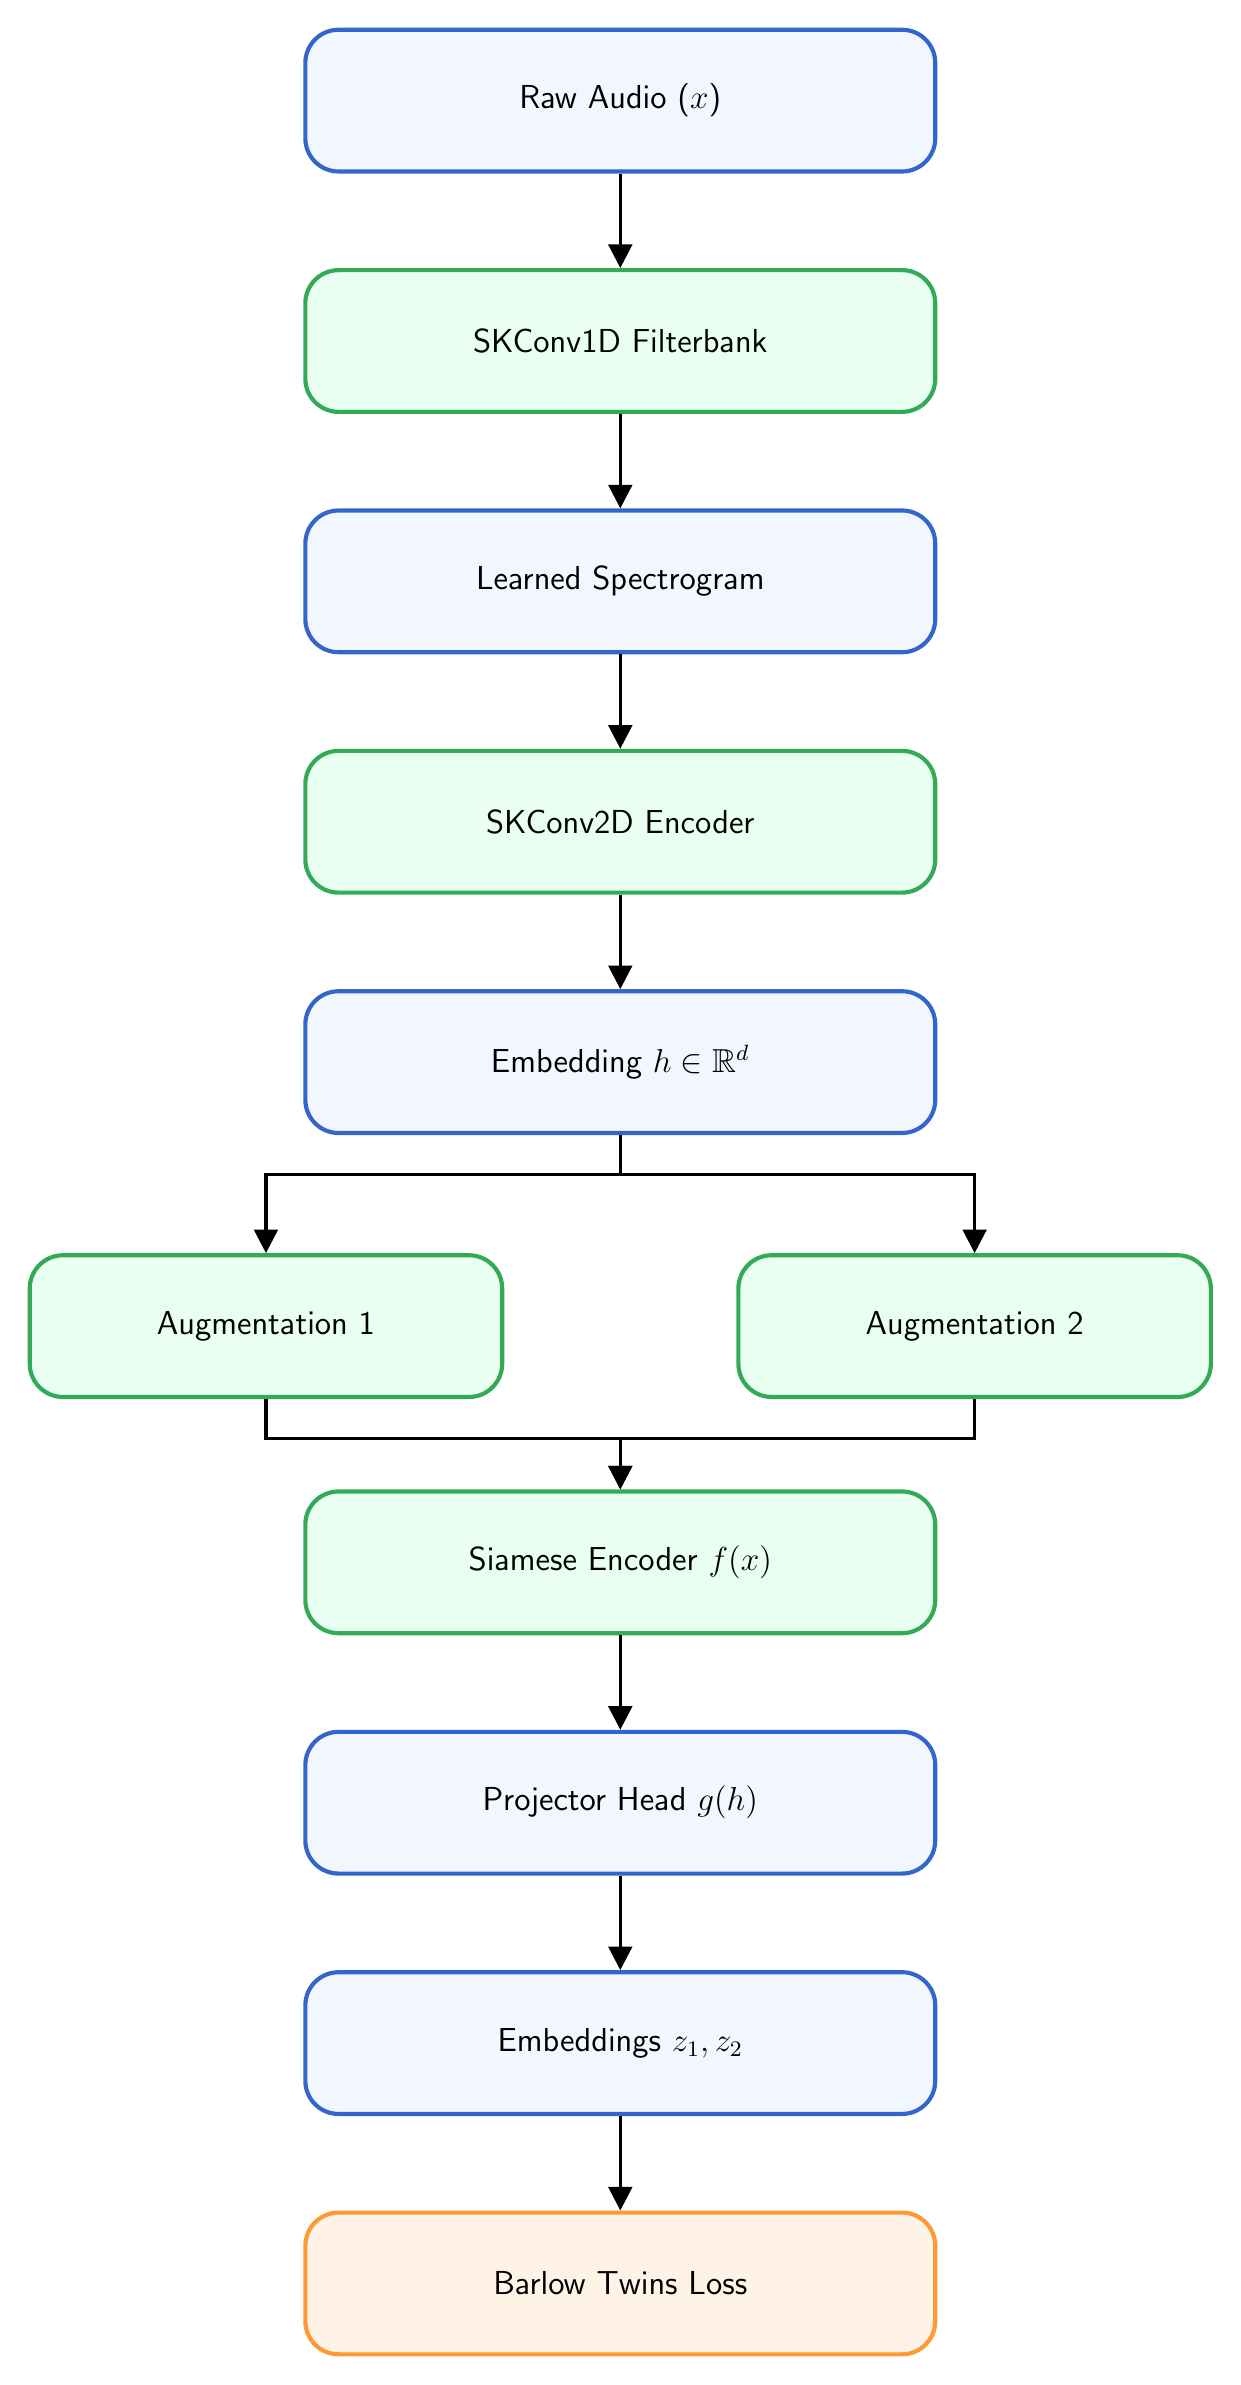
\begin{tikzpicture}[
    node distance=1.2cm,
    font=\sffamily\large,
    line width=1.5pt,
    box/.style={
        rectangle, rounded corners=12pt,
        draw=boxStroke, fill=boxFill,
        align=center, minimum width=8cm,
        minimum height=1.8cm, inner sep=10pt
    },
    proc/.style={
        rectangle, rounded corners=12pt,
        draw=procStroke, fill=procFill,
        align=center, minimum width=8cm,
        minimum height=1.8cm, inner sep=10pt
    },
    loss/.style={
        rectangle, rounded corners=12pt,
        draw=lossStroke, fill=lossFill,
        align=center, minimum width=8cm,
        minimum height=1.8cm, inner sep=10pt
    },
    arrow/.style={
        -{Triangle[length=3mm,width=3mm]},
        draw=black, line width=1.2pt
    }
]
    \node[box] (audio) {Raw Audio ($x$)};
    \node[proc, below=of audio] (filter) {SKConv1D Filterbank};
    \node[box, below=of filter] (spec) {Learned Spectrogram};
    \node[proc, below=of spec] (enc2d) {SKConv2D Encoder};
    \node[box, below=of enc2d] (emb) {Embedding $h \in \mathbb{R}^d$};

    \node[proc, below=1.5cm of emb, xshift=-4.5cm, minimum width=6cm] (aug1) {Augmentation 1};
    \node[proc, below=1.5cm of emb, xshift=4.5cm, minimum width=6cm] (aug2) {Augmentation 2};

    \node[proc, below=4.5cm of emb] (siam) {Siamese Encoder $f(x)$};
    \node[box, below=of siam] (proj) {Projector Head $g(h)$};
    \node[box, below=of proj] (z) {Embeddings $z_1, z_2$};
    \node[loss, below=of z] (lossnode) {Barlow Twins Loss};

    \draw[arrow] (audio) -- (filter);
    \draw[arrow] (filter) -- (spec);
    \draw[arrow] (spec) -- (enc2d);
    \draw[arrow] (enc2d) -- (emb);

    \draw[arrow] (emb.south) -- ++(0,-0.5) -| (aug1.north);
    \draw[arrow] (emb.south) -- ++(0,-0.5) -| (aug2.north);

    \draw[arrow] (aug1.south) -- ++(0,-0.5) -| (siam.north);
    \draw[arrow] (aug2.south) -- ++(0,-0.5) -| (siam.north);

    \draw[arrow] (siam) -- (proj);
    \draw[arrow] (proj) -- (z);
    \draw[arrow] (z) -- (lossnode);
\end{tikzpicture}
\end{adjustbox}
\caption{SKANN-SSL end-to-end pipeline.}
\end{figure}

% =================================================
\clearpage
\section*{13. Summary \& Conclusion (Non-Pipeline)}

A complete, modern, scalable self-supervised acoustic representation learning system.
Suitable for sonar, HAVS, machinery vibration, and environmental acoustics.
Industry-grade and implementation-ready.

\end{document}
